% moments / leading conjectured term (generated by review/volume15-rewrite/fig_ch10_ratios.py).
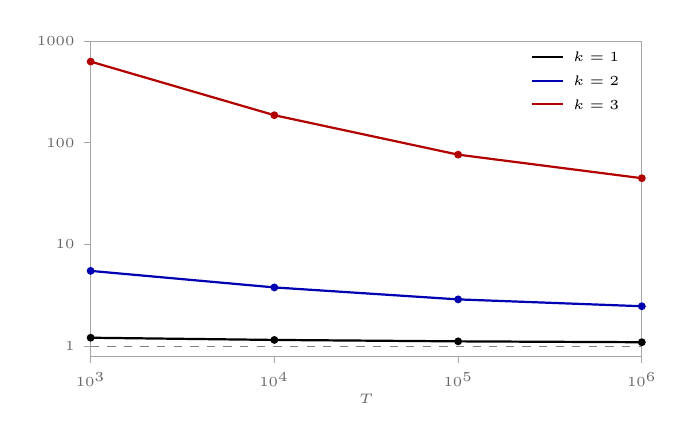
\begin{tikzpicture}[x=1cm,y=1cm]
\draw[black!35] (0,0) rectangle (7.00,4.00);
\draw[black!35] (0.00,0)--(0.00,-0.08) node[below,font=\tiny,black!60]{$10^3$};
\draw[black!35] (2.33,0)--(2.33,-0.08) node[below,font=\tiny,black!60]{$10^4$};
\draw[black!35] (4.67,0)--(4.67,-0.08) node[below,font=\tiny,black!60]{$10^5$};
\draw[black!35] (7.00,0)--(7.00,-0.08) node[below,font=\tiny,black!60]{$10^6$};
\draw[black!35] (0,0.13)--(-0.08,0.13) node[left,font=\tiny,black!60]{$1$};
\draw[black!35] (0,1.42)--(-0.08,1.42) node[left,font=\tiny,black!60]{$10$};
\draw[black!35] (0,2.71)--(-0.08,2.71) node[left,font=\tiny,black!60]{$100$};
\draw[black!35] (0,4.00)--(-0.08,4.00) node[left,font=\tiny,black!60]{$1000$};
\node[below,font=\tiny,black!60] at (3.50,-0.35) {$T$};
\draw[black!50,dashed] (0,0.13)--(7.00,0.13);
\draw[black,thick] (0.000,0.236) -- (2.333,0.208) -- (4.667,0.190) -- (7.000,0.179);
\fill[black] (0.000,0.236) circle (0.05cm);
\fill[black] (2.333,0.208) circle (0.05cm);
\fill[black] (4.667,0.190) circle (0.05cm);
\fill[black] (7.000,0.179) circle (0.05cm);
\draw[blue!70!black,thick] (0.000,1.085) -- (2.333,0.875) -- (4.667,0.723) -- (7.000,0.636);
\fill[blue!70!black] (0.000,1.085) circle (0.05cm);
\fill[blue!70!black] (2.333,0.875) circle (0.05cm);
\fill[blue!70!black] (4.667,0.723) circle (0.05cm);
\fill[blue!70!black] (7.000,0.636) circle (0.05cm);
\draw[red!70!black,thick] (0.000,3.743) -- (2.333,3.062) -- (4.667,2.561) -- (7.000,2.262);
\fill[red!70!black] (0.000,3.743) circle (0.05cm);
\fill[red!70!black] (2.333,3.062) circle (0.05cm);
\fill[red!70!black] (4.667,2.561) circle (0.05cm);
\fill[red!70!black] (7.000,2.262) circle (0.05cm);
\draw[black,thick] (5.60,3.80)--(6.00,3.80) node[right,font=\tiny,black]{$k=1$};
\draw[blue!70!black,thick] (5.60,3.50)--(6.00,3.50) node[right,font=\tiny,black]{$k=2$};
\draw[red!70!black,thick] (5.60,3.20)--(6.00,3.20) node[right,font=\tiny,black]{$k=3$};
\end{tikzpicture}
